% Antagonist phase geometry, generated from labeled_line_phase_lif_v3.json.
% Angle is the agonist/antagonist phase difference in cycles; radius is phase
% concentration across 30 Poisson realizations. Control panels are averaged over
% their graph seeds (circular mean for phase).
\documentclass[tikz,border=3pt]{standalone}
\usepackage[T1]{fontenc}
\usepackage{xcolor}
\usetikzlibrary{arrows.meta,calc}

\definecolor{ink}{HTML}{233747}
\definecolor{blue}{HTML}{256B91}
\definecolor{green}{HTML}{3A7D5D}
\definecolor{grey}{HTML}{68747D}

\begin{document}
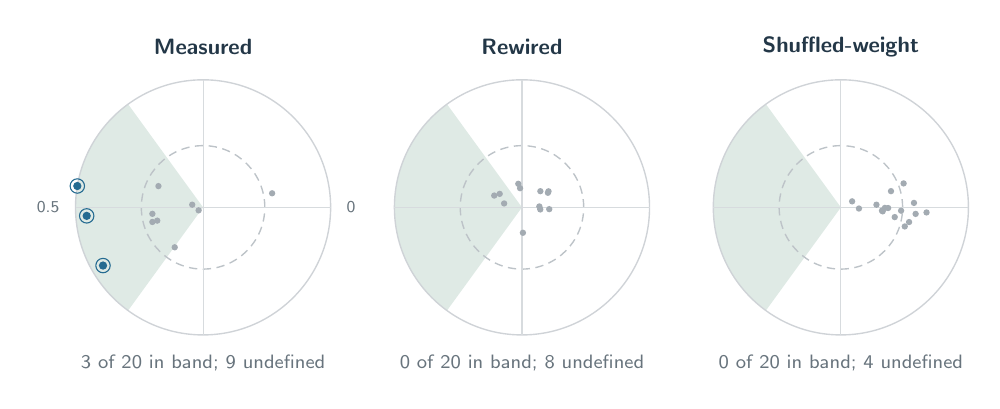
\begin{tikzpicture}[x=1cm,y=1cm]

%% ---- real ----
\begin{scope}[shift={(0.0,0)}]
\fill[green!16] (0,0) -- (126.0:1.62) arc [start angle=126.0, end angle=234.0, radius=1.62] -- cycle;
\draw[draw=ink!22,line width=.5pt] (0,0) circle [radius=1.62];
\draw[draw=ink!30,densely dashed,line width=.5pt] (0,0) circle [radius=0.784];
\draw[draw=ink!18,line width=.4pt] (0,0) -- (0:1.62);
\draw[draw=ink!18,line width=.4pt] (0,0) -- (90:1.62);
\draw[draw=ink!18,line width=.4pt] (0,0) -- (180:1.62);
\draw[draw=ink!18,line width=.4pt] (0,0) -- (270:1.62);
\fill[ink!42] (-125.38:0.622) circle [radius=1.15pt];
\fill[ink!42] (-172.74:0.649) circle [radius=1.15pt];
\fill[blue] (-175.82:1.482) circle [radius=1.5pt];
\draw[blue,line width=.4pt] (-175.82:1.482) circle [radius=2.6pt];
\fill[ink!42] (-163.86:0.606) circle [radius=1.15pt];
\fill[blue] (170.36:1.620) circle [radius=1.5pt];
\draw[blue,line width=.4pt] (170.36:1.620) circle [radius=2.6pt];
\fill[ink!42] (154.53:0.628) circle [radius=1.15pt];
\fill[ink!42] (-163.95:0.670) circle [radius=1.15pt];
\fill[ink!42] (11.53:0.895) circle [radius=1.15pt];
\fill[ink!42] (-146.29:0.068) circle [radius=1.15pt];
\fill[blue] (-149.82:1.470) circle [radius=1.5pt];
\draw[blue,line width=.4pt] (-149.82:1.470) circle [radius=2.6pt];
\fill[ink!42] (166.17:0.142) circle [radius=1.15pt];
\node[font=\sffamily\bfseries\fontsize{7.8}{9}\selectfont,text=ink] at (0,2.04) {Measured};
\node[font=\sffamily\fontsize{6.6}{7.6}\selectfont,text=grey] at (0,-1.98) {3 of 20 in band; 9 undefined};
\end{scope}

%% ---- rewired ----
\begin{scope}[shift={(4.05,0)}]
\fill[green!16] (0,0) -- (126.0:1.62) arc [start angle=126.0, end angle=234.0, radius=1.62] -- cycle;
\draw[draw=ink!22,line width=.5pt] (0,0) circle [radius=1.62];
\draw[draw=ink!30,densely dashed,line width=.5pt] (0,0) circle [radius=0.784];
\draw[draw=ink!18,line width=.4pt] (0,0) -- (0:1.62);
\draw[draw=ink!18,line width=.4pt] (0,0) -- (90:1.62);
\draw[draw=ink!18,line width=.4pt] (0,0) -- (180:1.62);
\draw[draw=ink!18,line width=.4pt] (0,0) -- (270:1.62);
\fill[ink!42] (31.14:0.394) circle [radius=1.15pt];
\fill[ink!42] (-3.77:0.347) circle [radius=1.15pt];
\fill[ink!42] (148.78:0.331) circle [radius=1.15pt];
\fill[ink!42] (29.34:0.378) circle [radius=1.15pt];
\fill[ink!42] (156.91:0.383) circle [radius=1.15pt];
\fill[ink!42] (-87.88:0.323) circle [radius=1.15pt];
\fill[ink!42] (-6.44:0.234) circle [radius=1.15pt];
\fill[ink!42] (3.06:0.221) circle [radius=1.15pt];
\fill[ink!42] (98.88:0.303) circle [radius=1.15pt];
\fill[ink!42] (41.36:0.311) circle [radius=1.15pt];
\fill[ink!42] (95.68:0.245) circle [radius=1.15pt];
\fill[ink!42] (167.66:0.232) circle [radius=1.15pt];
\node[font=\sffamily\bfseries\fontsize{7.8}{9}\selectfont,text=ink] at (0,2.04) {Rewired};
\node[font=\sffamily\fontsize{6.6}{7.6}\selectfont,text=grey] at (0,-1.98) {0 of 20 in band; 8 undefined};
\end{scope}

%% ---- random ----
\begin{scope}[shift={(8.1,0)}]
\fill[green!16] (0,0) -- (126.0:1.62) arc [start angle=126.0, end angle=234.0, radius=1.62] -- cycle;
\draw[draw=ink!22,line width=.5pt] (0,0) circle [radius=1.62];
\draw[draw=ink!30,densely dashed,line width=.5pt] (0,0) circle [radius=0.784];
\draw[draw=ink!18,line width=.4pt] (0,0) -- (0:1.62);
\draw[draw=ink!18,line width=.4pt] (0,0) -- (90:1.62);
\draw[draw=ink!18,line width=.4pt] (0,0) -- (180:1.62);
\draw[draw=ink!18,line width=.4pt] (0,0) -- (270:1.62);
\fill[ink!42] (-3.39:1.090) circle [radius=1.15pt];
\fill[ink!42] (-16.62:0.847) circle [radius=1.15pt];
\fill[ink!42] (20.89:0.853) circle [radius=1.15pt];
\fill[ink!42] (-4.99:0.953) circle [radius=1.15pt];
\fill[ink!42] (17.92:0.669) circle [radius=1.15pt];
\fill[ink!42] (3.49:0.930) circle [radius=1.15pt];
\fill[ink!42] (-4.53:0.524) circle [radius=1.15pt];
\fill[ink!42] (-3.69:0.230) circle [radius=1.15pt];
\fill[ink!42] (-12.15:0.886) circle [radius=1.15pt];
\fill[ink!42] (-0.81:0.600) circle [radius=1.15pt];
\fill[ink!42] (4.29:0.453) circle [radius=1.15pt];
\fill[ink!42] (28.14:0.162) circle [radius=1.15pt];
\fill[ink!42] (-3.18:0.766) circle [radius=1.15pt];
\fill[ink!42] (-0.70:0.559) circle [radius=1.15pt];
\fill[ink!42] (-5.43:0.533) circle [radius=1.15pt];
\fill[ink!42] (-10.24:0.695) circle [radius=1.15pt];
\node[font=\sffamily\bfseries\fontsize{7.8}{9}\selectfont,text=ink] at (0,2.04) {Shuffled-weight};
\node[font=\sffamily\fontsize{6.6}{7.6}\selectfont,text=grey] at (0,-1.98) {0 of 20 in band; 4 undefined};
\end{scope}
\node[font=\sffamily\fontsize{6.2}{7.2}\selectfont,text=grey,anchor=west] at (1.70,0) {0};
\node[font=\sffamily\fontsize{6.2}{7.2}\selectfont,text=grey,anchor=east] at (-1.70,0) {0.5};
\end{tikzpicture}
\end{document}
